\textbf{2-1} 如光图2-1-1所示，汽车B沿公路由东向西作匀速直线运动。路南房子H中--电视机正在接收从西南远方传来的频率为 $f = 60\mathrm{MHz}$ 的电磁波。房子H到公路的垂直距离 $L = 100$ m。汽车驶过房子所在地区时，电视机接收到的信号强度将发生起伏。当汽车处于正对房子的位置时，测得强度起伏频率为 $2\mathrm{Hz}$ ；当汽车离正对位置距离为 $200\mathrm{m}$ 时，起伏频率突然降为零。试求电磁波的发射方位及汽车的行驶速度 $\pmb{\nu}$ 。


\begin{center}
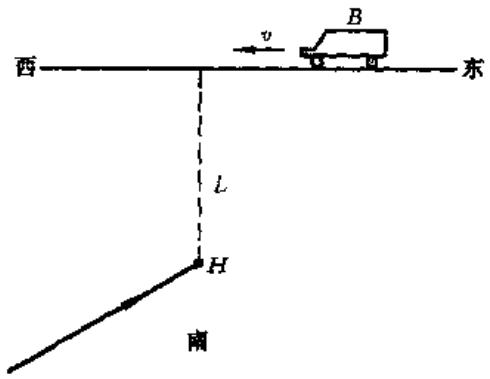
\includegraphics[width=0.3\textwidth]{figures/光图2-1-1.jpg}
\end{center}
\vfill

\textbf{2-2}某射电天文台的接收天线位于海平面上方高度为 $h = 2.00\mathrm{m}$ 处，接收机只记录电场强度的水平分量。当一颗能发射波长为 $\lambda = 21.0\mathrm{cm}$ 电磁波的射电星从海平面升起时，接收机将相

继地记录下一系列极大值和极小值.

1. 试确定观察到极大值和极小值时电磁波的方向, 用与海平面的夹角表示该方向.

2. 当射电星从海平面上方出现时, 试间接收到的电磁波的强度是增加还是减小?

3. 试求观察到的相继各极大值与极小值的相对强度.
\begin{center}
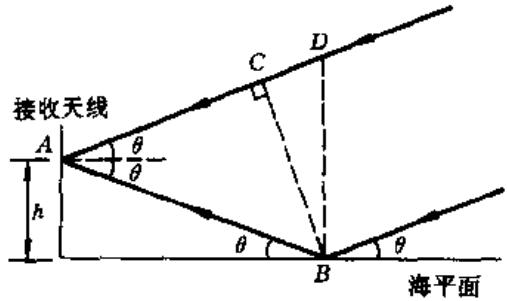
\includegraphics[width=0.3\textwidth]{figures/光图2-2-1.jpg}
\end{center}

\vfill
\textbf{2-3} 如光图2-3-1所示，已知菲涅耳双面镜两镜之间的夹角 $\alpha = 20^{\prime}$ ，缝光源与两镜交线的距离 $R =$

10 cm, 单色光的波长 $\lambda = 600 \, nm$ , 观察屏幕与两虚光源的连线平行, 与两镜交线相距 L = 210 cm.

试问:1. 幕上干涉条纹的间距多大? 在幕上最多能看到多少条干涉条纹? 2. 若光源到两镜

交线的距离增大一倍,干涉条纹怎样变化?3.若缝光源横向移动 $\delta s$ ,干涉条纹如何变化?4.为了能观察到干涉条纹,光源的极限宽度为多大?

\vfill
\newpage
\textbf{2-4} 如光图2-4-1所示，焦距 $f = 10\mathrm{cm}$ 的薄透镜沿其直径剖切为二，再沿切口的垂直方向将两半移

开一距离 $\delta=1.0\ mm$ . 在透镜前方, 在对称轴上与透镜相距为 s=20 cm 处放一单色点光源 Q, 其波长 $\lambda=500\ nm$ , 在透镜另一侧与透镜相距为 L=50 cm 处, 与对称轴垂直地放一屏幕. 试求幕上出现的干涉条纹的数目.

\vfill
\textbf{2-5} 如光图2-5-1所示，在杨氏干涉装置中，用三个平行狭缝代替双缝，三缝的缝宽相同 $\left(\text{都} < \frac{\lambda}{2}\right)$ ，缝距分别为 $d$ 和 $\frac{3}{2} d$ ，设单色缝光源与三狭缝的距离足够远，因而到三缝的光程可看作相同，设幕与三缝的距离 $D$ 也足够远。试求：1.幕中心小范围内的强度随 $\theta$ 变化的分布公式。2.一级极大的角位置 $\theta_1$ .3.在 $\theta = \frac{\theta_1}{2}$ 方向的强度与一级极大强度之比。


\begin{center}
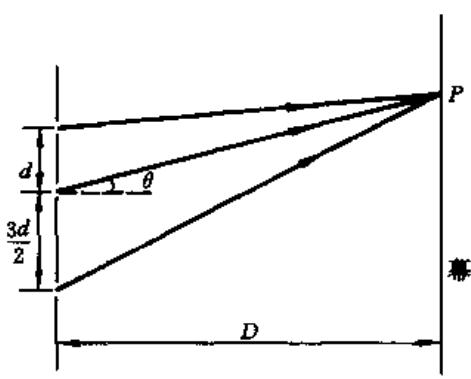
\includegraphics[width=0.3\textwidth]{figures/光图2-5-1.jpg}
\end{center}

\vfill
\newpage
\textbf{2-6} 波长均为 $\lambda$ ，振幅比为2:1的两相干平行光束，以 $\theta$ 的夹角射入，观察屏幕与 $\theta$ 角的角平分线相垂直.试求：1.幕上干涉条纹的反衬度.2.干涉条纹的间距.

\vfill
\textbf{2-7} 波长 $\lambda = 632.8\mathrm{nm}$ 的平行激光束垂直入射到双棱镜上，双棱镜的顶角 $\alpha = 3'30''$ ，宽度 $W = 4.0~\mathrm{cm}$ ，折射率 $n = 1.5$ 。试问：当幕与双棱镜的距离 $L$ 分别为多大时，在幕上观察到的干涉条纹的总数最少和最多？最多时能看到几条干涉条纹？

\vfill
\newpage
\textbf{2-8} 如图2-8-1所示，三束波长均为 $\lambda$ 的平面波沿 $xz$ 平面入射到位于 $z = 0$ 平面的屏幕上，它们的波矢分别为 $\pmb{K}_1, \pmb{K}_2$ 和 $\pmb{K}_3$ ，其中 $\pmb{K}_2$ 与 $z$ 轴一致， $\pmb{K}_1$ 和 $\pmb{K}_3$ 与 $z$ 轴夹角为 $\theta$ ，振幅依次为 $A_0, 2A_0$ 和 $A_0$ ，在坐标原点 $O$ 的初相位均为零.

试在以下三种情形下求幕上的干涉强度分布,条纹的反衬度和条纹间距.1. $K_{1}$ , $K_{2}$ 和 $K_{3}$ 波同时存在.2.只存在 $K_{1}$ 和 $K_{3}$ 波.3.只存在 $K_{1}$ 和 $K_{2}$ 波.试比较三种情形的干涉条纹特性.

\begin{center}
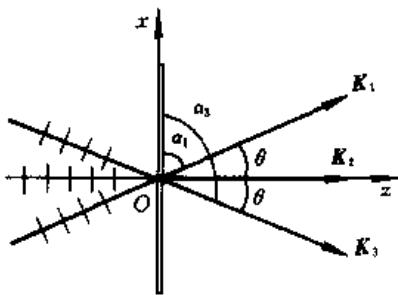
\includegraphics[width=0.25\textwidth]{figures/光图2-8-1.jpg}
\end{center}
\vfill
\textbf{2-9} 如光图2-9-1所示，一波矢为 $k$ ，振幅为 $A$ 的简谐平面波沿 $+z$ 方向传播.同时在 $z$ 轴上 $O$ 点处有一同频率的点波源发出简谐球面波.在与 $O$ 点距离为 $D$ 处放置一个与 $z$ 轴垂直的幕.假定平

面波与球面波在 O 点有相同的初相位, 球面波在与点波源 O 点的距离为一个单位长度处的振幅是平面波振幅的 D 倍, 幕与 z 轴交点处的光强为 $I_{0}$ . 试求幕上近轴区域干涉强度的分布公式, 干涉条纹的特征如何?
\begin{center}
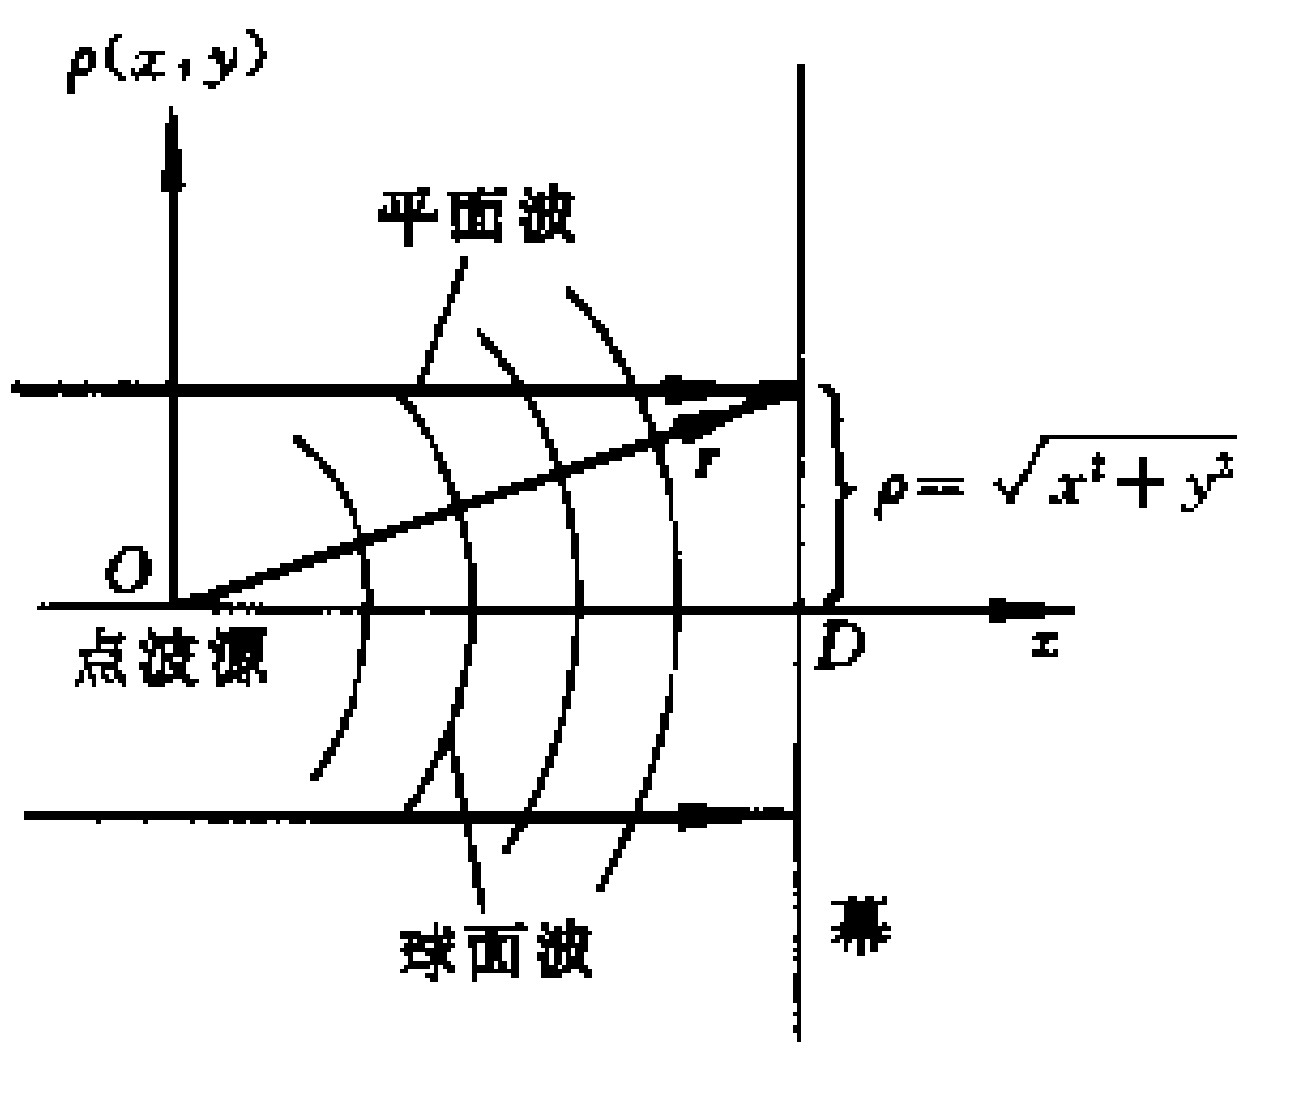
\includegraphics[width=0.3\textwidth]{figures/光图2-9-1.jpg}
\end{center}
\vfill
\newpage
\textbf{2-10} 如光图2-10-1的梅斯林干涉装置是将一透镜对剖后沿主光轴错开一定距离. 单色点光源 $S$ 位于主光轴上, 经上和下两个半透镜成像于 $S_{1}^{\prime}$ 和 $S_{2}^{\prime}$ , 在两束相干光的重叠区域内, 垂直于主光轴放一屏幕.

1. 试问在幕上的干涉条纹是什么形状？2. 设透镜焦距 $f = 30 \mathrm{~cm}$ . 点光源与较近的半透镜 $L_{1}$ 的距离为 $60 \mathrm{~cm}$ ，两个半透镜之间错开的距离为 $8.0 \mathrm{~cm}$ ，单色光的波长为 $500 \mathrm{~nm}$ ，屏幕放在

$S_{1}^{\prime}$ 和 $S_{2}^{\prime}$ 的中点. 试求在傍轴条件下幕上干涉条纹的间距.
\begin{center}
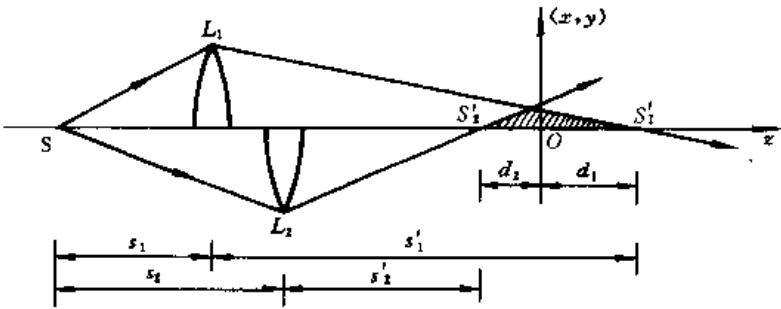
\includegraphics[width=0.5\textwidth]{figures/光图2-10-1.jpg}
\end{center}
\vfill
\textbf{2-11} 如光图2-11-1的洛埃镜镜长 $B - 5.00\mathrm{cm}$ ，幕与镜的右端相距 $C = 5.00\mathrm{m}$ ，点光源高出镜面的距离为 $d = 0.500\mathrm{mm}$ ，与镜左端的水平距离 $A = 2.00\mathrm{cm}$ ，光波波长 $\lambda = 600\mathrm{nm}$ .

1. 试求幕上干涉条纹的间距.2. 试问幕上总共能出现多少条干涉条纹.3. 为了在叠加区域能看到全部干涉条纹, 试问对光谱宽度 $\Delta \lambda$ 有何要求.
\begin{center}
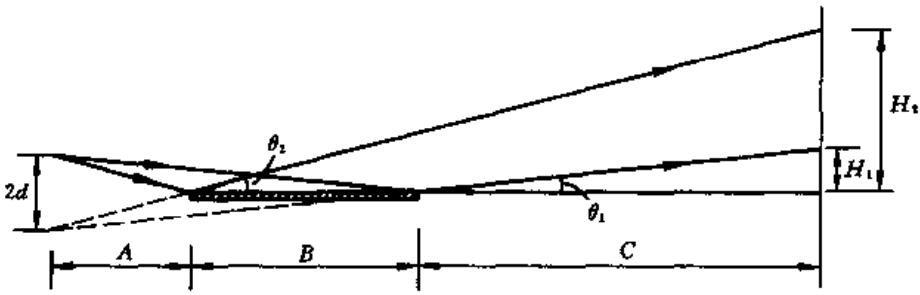
\includegraphics[width=0.5\textwidth]{figures/光图2-11-1.jpg}
\end{center}
\vfill
\newpage
\textbf{2-12} 如光图2-12-1所示，间距为 $d$ 的双孔 $\mathbf{S}_1$ 和 $\mathbf{S}_2$ 后放置一会聚透镜，透镜后焦面上放一屏幕.上述干涉装置正对遥远的双星S和 $\mathbf{S}'$ ，在幕上观察双星产生的干涉条纹.当 $d$ 从小连续变大时，干涉条纹的反衬度将作周期性变化.

1. 试解释此现象.2. 若星光的平均波长为 $550\mathrm{nm}$ , 当 $d$ 变到 $2.0\mathrm{mm}$ 时, 条纹第一次变模糊, 试求双星的角间距.


\begin{center}
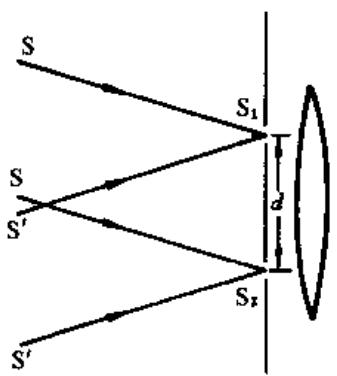
\includegraphics[width=0.2\textwidth]{figures/光图2-12-1.jpg}
\end{center}

\vfill
\textbf{2-13} 在杨氏干涉实验中，已知双孔间的距离为 $d$ ，光源到双孔的距离为 $R$ ，双孔到观察屏幕的距离为 $D$ ，单色光源的波长为 $\lambda$

试求:1. 屏幕上干涉条纹的反衬度 $\gamma$ 与光源宽度 b 之间的关系.2. 当光源宽度等于临界宽度的 $\frac{1}{4}$ 时, 干涉条纹有足够的反衬度, 此时 $\gamma$ 等于多少?

\vfill
\newpage
\textbf{2-14} 如光图2-14-1所示，间距为 $d$ 的双孔 $\mathbf{S}_1$ 和 $\mathbf{S}_2$ 后放置一会聚透镜，透镜后焦面上放一屏幕(与本章题12的装置相同).该干涉装置正对远处的扩展光源.试导出计算条纹反衬度的一般公式，并将此一般公式应用于发光强度均匀的矩形扩展光源.


\begin{center}
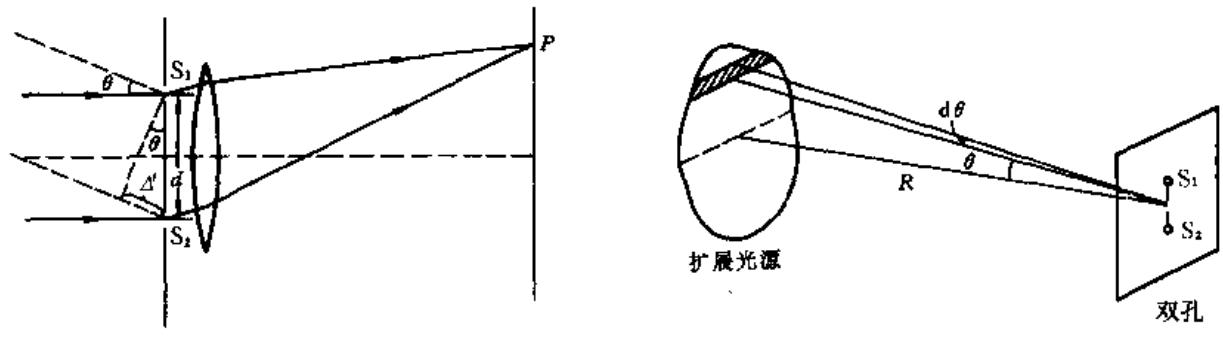
\includegraphics[width=0.6\textwidth]{figures/光图2-14-1.jpg}
\end{center}

\vfill
\textbf{2-15} 三个平凸透镜A、B、C，两两组合成牛顿环干涉装置.以波长 $\lambda = 600\mathrm{nm}$ 的单色光垂直入射，观察空气层产生的牛顿环.当A和B组合时，测得第10个暗环的半径为 $r_{AB} = 4.0\mathrm{mm}$ ；当B和C组合时，第10个暗环的半径为 $r_{BC} = 4.5\mathrm{mm}$ ；当C和A组合时，第10个暗环的半径为 $r_{CA} = 5.0\mathrm{mm}$ .设透镜两两组合时接触良好.试求：三个透镜球面的曲率半径 $R_{\mathrm{A}},R_{\mathrm{B}}$ 和 $R_{\mathrm{C}}$

\vfill
\newpage
\textbf{2-16} 沿着与楔形薄膜的法线成 $\theta_{i}$ 角的方向观察薄膜表面 $P$ 点附近的等厚干涉条纹. 设薄膜折射率为 $n, P$ 点处薄膜的厚度为 $t$ , 所用单色光波长为 $\lambda$ , 为使干涉条纹有足够的反衬度, 同一观察点光程差的差别不得大于 $\frac{\lambda}{4}$ .

1. 试问对光源宽度有何限制？

2. 若用眼睛直接观察干涉条纹，试问对薄膜厚度 $t$ 有何限制？已知 $n = 1.5, \theta_{i} = 30^{\circ}$ ，瞳孔直径 $D = 3 \mathrm{~mm}$ ，眼睛到 $P$ 点的距离 $L = 30 \mathrm{~cm}$ ，单色光波长 $\lambda = 550 \mathrm{~nm}$ ，薄膜放在空气中，空气折射率 $n_{0} = 1$ 。

\vfill
\textbf{2-17} 钠黄光是由波长为 $\lambda_{1}$ 和 $\lambda_{2}$ 的两条谱线组成的，平均波长为 $589.3\mathrm{nm}$ . 现用钠黄光观察迈克耳孙干涉仪的圆形条纹. 当连续移动一臂中的平面镜时, 干涉条纹从清晰到模糊, 又到清晰周期性地变化. 观察视场中某固定点, 测出从最清晰到第一次变为最模糊的过程中, 经该点移动了 490 条干涉条纹. 试求钠黄光中两波长的波长差.

\vfill
\newpage
\textbf{2-18} 用钠黄光 $(\lambda = 589.3\mathrm{nm})$ 观察迈克耳孙干涉仪的等倾圆条纹，开始时视场中共看到10个亮环，中心为亮斑，然后移动干涉仪一臂的平面镜，先后看到共有10个亮环缩进中央，而视场中除中心为亮斑外，还剩下5个亮环.

试求:1. 平面镜移动的距离.

2. 开始时中心亮斑的干涉级次.

3. 移动平面镜后最外一个亮环的干涉级次.

\vfill
\textbf{2-19} 迈克耳孙干涉仪一臂中的反射镜以均匀速度 $v$ 平行移动.用透镜将干涉条纹成像于光电元件的取样窗上，条纹移动时，进入取样窗的光强的变化将转换成电信号的变化.

1. 若光源波长 $\lambda = 600 \, nm$ ，测得电信号变化的时间频率为 $\nu = 50 \, Hz$ 。试求反射镜移动的速度。

2. 若以平均波长为 $589.3 \, nm$ 的钠黄光作光源，反射镜平行移动的速度取第 1 问的数值，测得电信号的拍频频率为 $5.2 \times 10^{-2} \, Hz$ 。试求钠黄光中两谱线的波长差。

\vfill
\newpage
\textbf{2-20} 法布里－珀罗干涉仪可产生强而锐的干涉条纹，故常用来测量波长差很小的两谱线的波长差。如光图2-20-1设平均波长为 $\overline{\lambda} = 500\mathrm{nm}$ 的某谱线由波长差为 $\lambda_{1}$ 和 $\lambda_{2}$ 的两条谱线组成，干涉仪两板的间距为 $h = 0.25\mathrm{mm}$ ，波长为 $\lambda_{1}$ 的第2和第5干涉环的半径分别为 $2.00\mathrm{mm}$ 和3.80 mm，波长为 $\lambda_{2}$ 的第2和第5干涉环的半径分别为2.10 mm和3.85 mm。试求两谱线的波长差。
\begin{center}
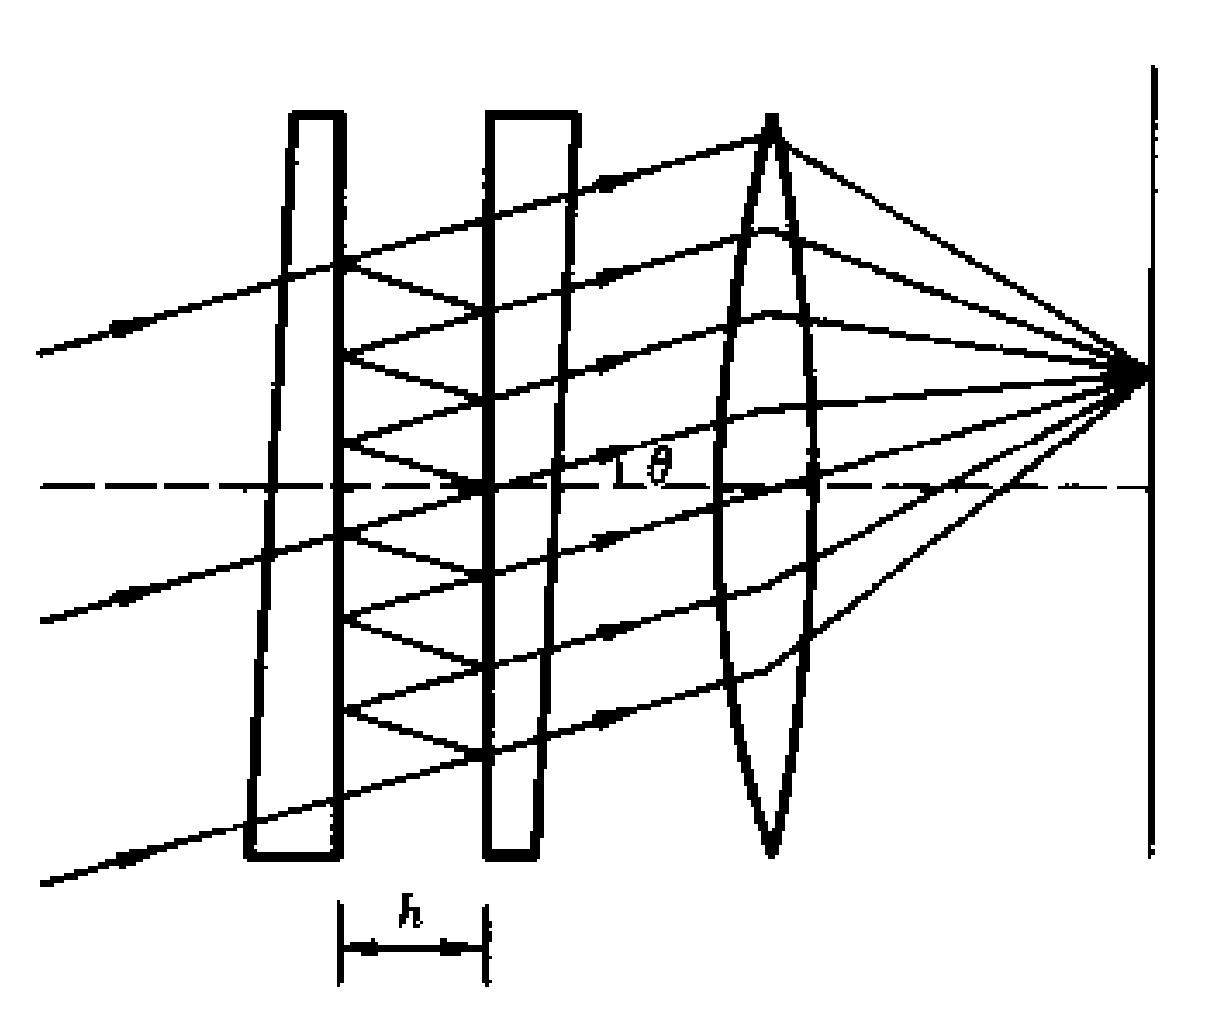
\includegraphics[width=0.2\textwidth]{figures/光图2-20-1.jpg}
\end{center}
\vfill
\textbf{2-21} 法布里-珀罗干涉仪的干涉强度 $I$ 随相邻两相干光之间的相位差 $\delta$ 变化.在如光图2-24-1所示的 $I(\delta)$ 曲线中，若干涉极大的半强度的宽度用 $\varepsilon$ 表示，定义条纹的锐度系数为
$$ F = \frac {1 6}{\varepsilon^ {2}} $$
定义条纹的锐度为
$$ S = \frac {2 \pi}{\varepsilon} $$
1. 试求锐度系数和锐度与反射率 R 之间的关系. 

2. 已知某法布里－珀罗干涉仪金属涂层的反射系数 r = 0.894. 试求条纹的半强度宽 $\epsilon$ , 锐度系数 F 以及锐度 S.
\begin{center}
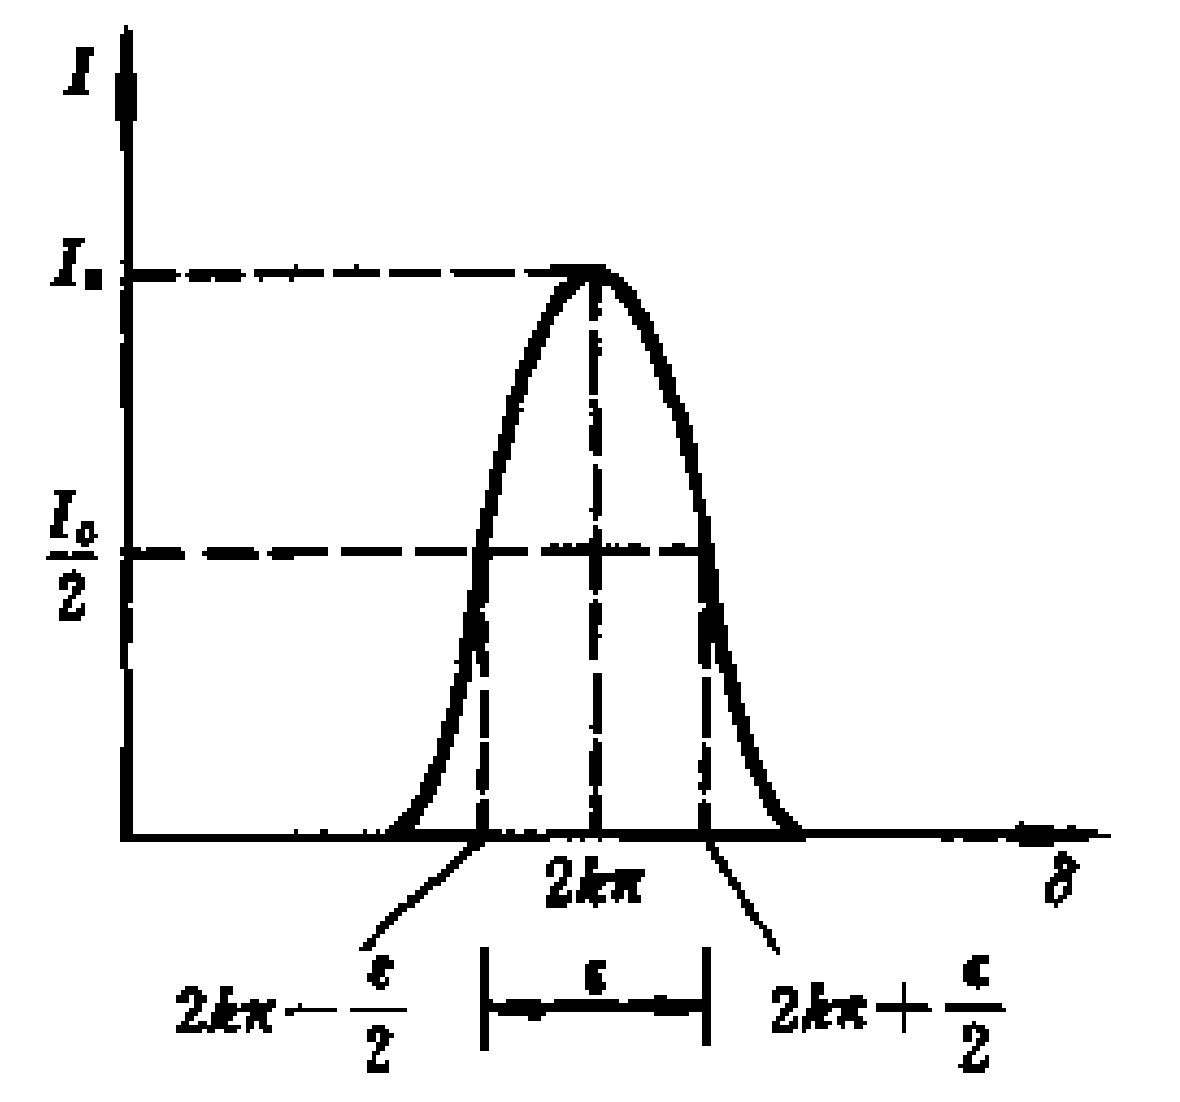
\includegraphics[width=0.2\textwidth]{figures/光图2-21-1.jpg}
\end{center}

\vfill
\newpage
\textbf{2-22} 激光器谐振腔的两平行反射镜可看作是一个法布里-珀罗标准具.

1.试导出激光器输出的频率间隔公式.

2.试导出谱线宽度的公式(分别以频率和波长表示宽度).

3.已知一个He-Ne(氦-氖)激光器的腔长 $h = 0.50\mathrm{m}$ .两反射镜的反射率 $R = 0.99$ .试问输出激光的频率间隔和谐线宽度各是多少？设气体折射率 $n = 1$ ，输出激光的中心波长为 $\lambda = 632.8\mathrm{nm}$

\vfill
\textbf{2-23} 平行平面薄膜的折射率 $n = 1.5$ ，放置在空气中.单色光近乎垂直入射.在垂直于薄膜的方向用望远镜分别观察反射光和透射光的等倾干涉图样.试求两种干涉条纹的反衬度(不计多重反射).

\vfill
\newpage
\textbf{2-24} 在折射率 $n_{\mathrm{g}} = 1.50$ 的玻璃平板表面涂一层折射率 $n_{\mathrm{f}} = 1.38$ 的氟化镁. 波长 $\lambda = 550 \mathrm{~nm}$ 的单色光从空气垂直入射.试求:

1. 为使反射光干涉相消, 氟化镁涂层的最小厚度为多少? 与不加涂层相比, 此时光强反射率降低了多少? 

2. 取第1问的涂层厚度, 对波长为400 nm 和700 nm 的光来说, 光强反射率如何?

\vfill


\textbf{2-25} 如光图2-25-1所示,砷化镓发光管常制成半球形,以减少位于球心的发光区向外输出功率时的反射损失.为了进一步提高输出光功率常在球形表面涂一层增透膜.砷化镓发光管发光波长 $\lambda = 930\mathrm{nm}$ ，砷化镓的折射率 $n_1 = 3.4$ ，空气折射率 $n_2\approx 1$.试问:

1. 不涂增透膜时球面的光强反射率为多大? 

2. 为使反射光完全干涉相消, 增透膜的厚度和折射率应取多大? 

3. 涂层分别用氟化镁(折射率为 1.38) 和硫化锌(折射率为 2.38) 时, 球面的光强反射率各为多少? 能否达到增透的目的?

\begin{center}
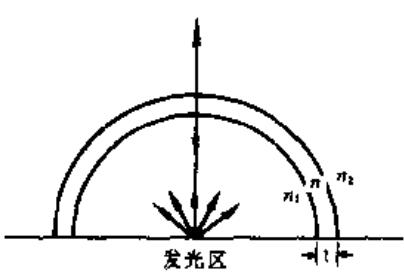
\includegraphics[width=0.3\textwidth]{figures/光图2-25-1.jpg}
\end{center}
\vfill
\newpage






\textbf{2-26} 在玻璃基片上涂一层薄膜，薄膜的折射率为 $n$ ，玻璃的折射率为 $n_{\mathrm{G}}$ ，另一侧是空气，折射率为 $n_0$

1. 试证明单色光正入射时, 光强反射率为
$$ R = \frac {(n _ {0} - n _ {G}) ^ {2} \cos^ {2} \frac {\delta}{2} + \left(\frac {n _ {0} n _ {G}}{n} - n\right) ^ {2} \sin^ {2} \frac {\delta}{2}}{(n _ {0} + n _ {G}) ^ {2} \cos^ {2} \frac {\delta}{2} + \left(\frac {n _ {0} n _ {G}}{n} + n\right) ^ {2} \sin^ {2} \frac {\delta}{2}} $$
式中
$$ \delta = \frac {4 \pi}{\lambda} n h $$
$h$ 是薄膜的厚度.

2. 试问,为使薄膜对某一波长的光起完全消反射的作用,薄膜的厚度和折射率应满足什么条件?

3. 如光图 2-26-1 所示, 若在折射率为 $n_{\mathrm{G}}$ 的基片上, 依次涂上高折射率层 $(n_{\mathrm{H}})$ 和低折射率层 $(n_{\mathrm{L}})$ , 每层的光学厚度均为 $\frac{\lambda}{4}$ . 试问, 为了达到完全消反射, $n_{\mathrm{H}}$ 和 $n_{\mathrm{L}}$ 应满足什么条件?


\begin{center}
    \begin{tabular}{ll}
        空气 & $n_0$ \\
        \hline
        低折射率层 & $n_{\mathrm{L}}$ \\
        \hline
        高折射率层 & $n_{\mathrm{H}}$ \\
        \hline
        基片 & $n_{\mathrm{G}}$ \\
    \end{tabular}
\end{center}


\vfill
\newpage

\textbf{2-27} 如光图2-27-1所示,多层高反射膜由光学厚度均满足干涉相消条件的高折射率层(如硫化锌)和低折射率层(如氟化镁)交替重叠而成.与玻璃基片和空气相邻的是高折射率层,故高反射膜的层数是奇数.

1. 已知空气折射率为 $n_{0}$ ，玻璃折射率为 $n_{G}$ ，高折射率层和低折射率层的折射率分别是 $n_{H}$ 和 $n_{L}$ ，总的层数为 $(2k+1)$ 。试证明，在正入射条件下，多层膜的光强反射率为
$$ R _ {2 k + 1} = \left[ \frac {n _ {0} - \left(\frac {n _ {\mathrm{H}}}{n _ {\mathrm{L}}}\right) ^ {2 k} \frac {n _ {\mathrm{H}} ^ {2}}{n _ {\mathrm{G}}}}{n _ {0} + \left(\frac {n _ {\mathrm{H}}}{n _ {\mathrm{L}}}\right) ^ {2 k} \frac {n _ {\mathrm{H}} ^ {2}}{n _ {\mathrm{G}}}} \right] $$
2. 若 $n_{0}=1, n_{G}=1.50, n_{H}=2.40, n_{L}=1.38$ . 试计算五层膜和九层膜的反射率.


\begin{center}
    % 将第一个列格式改为 p{2cm}，你可以将 2cm 修改为你需要的具体宽度
    \begin{tabular}{|>{\centering\arraybackslash}p{4cm}l|}
        \multicolumn{1}{>{\centering\arraybackslash}p{4cm}}{空气} & \multicolumn{1}{l}{$n_0$} \\
        \hline
          & $n_{\mathrm{H}}$ \\
        \hline
          & $n_{\mathrm{L}}$ \\
        \hline
          & $n_{\mathrm{H}}$ \\
        \hline
          & $n_{\mathrm{L}}$ \\
        \hline
          & $n_{\mathrm{H}}$ \\
        \hline
          & $n_{\mathrm{L}}$ \\
        \hline
          & $n_{\mathrm{H}}$ \\
        \hline
        玻璃 & $n_{\mathrm{G}}$ \\
         & 
    \end{tabular}
\end{center}


\vfill
